\documentclass[12pt]{article}

\usepackage{float, graphicx}
\usepackage[margin=2.5cm]{geometry}
\usepackage{amsmath, amsthm, amssymb}
\usepackage{wrapfig}
\usepackage[lined,boxed,commentsnumbered]{ algorithm2e }
\graphicspath{ { ./img/ } }
\newtheorem{definition}{Definition}

\usepackage{setspace}
\doublespacing

% Allows us to write code in the text %
\def\code#1{\texttt{#1}}

\begin{document}

\begin{titlepage}
	\begin{center}
		~\\[2.0cm]
		{\Huge Simulating Detachment of Tumor Cell Clusters}\\[1.5cm]
		{\Large HGEN 396: Human Genetics Research Project}\\[6.5cm]
		\emph{Student:}\\
		Mr. Zafarali Ahmed (260560472)\\
		{\scriptsize zafarali [dot] ahmed [at] mail [dot] mcgill [dot] ca} \\[1.0cm]
		\emph{Supervisor:}\\
		Dr. Simon Gravel\\[1.0cm]
		\emph{Submission Date:}\\
		\today\\[1.0cm]
		\emph{Location:}\\
		McGill University
	\end{center}
\end{titlepage}

\begin{abstract}
Blood of patients with cancer contain Circulating Tumor Cells (CTCs). CTCs are the primary method through which metastasis can occur. Advances in capture technology find that CTCs exist in single cells as well as in clusters. While both contribute to metastasis, clusters have an elevated metastatic potential \cite{Aceto2014}. Rarity of CTCs make it difficult to study \emph{in vivo} and \emph{in vitro} studies are challenging to design. \\
However, we can use toy models to study them \emph{in silico}. This paper primarily looks at the suitability and the feasibility of the Cellular Potts Model (CPM) to achieve this. We simulate a range of cluster sizes and compare their properties. We also separate a tissue in two by applying opposing forces to the mass of cells. We conclude that the model selected is a clean and informative tool that can provide us with new insights into CTC formation.
\end{abstract}

\section{Introduction}
Cancer is the autonomous and uncontrolled growth of cells that forms a feed forward system to reinforce the tumors’ existence \cite{hallmarks}. Cancer originates from accumulated mutations in tumor supressor genes, proto-onco genes and DNA repair genes. These mutations hinder a cell's abillity to regulate its cell cycles, causing it to divide uncontrollably. However, for cancerous cells to keep growing and overcome the limitations of efficient diffusion of nutrients, tumors have two solutions: angiogenesis and metastasis. Angiogenesis permits a tumor to grow blood vessels and bring in nutrients. Metastasis is the migration of cancer cells to other parts of the body often via the permeable blood vessels formed during angiogenesis. It is often after metastasis that cancer becomes difficult to contain and treat despite surgical resection \cite{Demicheli2008}.

For the tumor cells to perform invasion - the first step in metastasis - the migrating cell must alter its surface interactions with the microenvironment: neighboring cells and the extra cellular matrix. Altered expression of cell adhesion molecules like cadherins and catenins facilitate these changes in interactions \cite{Aktary2012}\cite{Zhurinsky2000}. Once the escaped tumor cell enters the blood stream, it is referred to as a \emph{Circulating Tumor Cell} (CTC).

In a recent study \cite{Aceto2014}, CTC-Chip and CTC-iChip isolation of blood from patients with breast cancer, verified the existence of both single-CTCs and CTC-clusters. Despite being rare,  clusters demonstrated (i) higher metastatic potential, (ii) faster disease progression than their single celled counterparts and were found to (iii) originate directly from the tumor rather than aggregate in the blood.

The study also attributed the elevated expression of \emph{plakoblogin} to the formation of clusters. A literature review for plakoglobin reveals opposing schools of thought because its role in cancer and metastasis is not completely understood \cite{Aktary2012}\cite{Zhurinsky2000}.

Capturing the above tumor dynamics, we attempt to use the Cellular Potts Model to simulate and investigate parameters resulting in the formation of single-CTCs and CTC-clusters.

\section{Purpose and Objectives}
Since metastasis is the \emph{point of no return} for most patients, it is necessary to build intuition of the factors that influence the production of single-CTCs versus CTC-clusters and the sizes of CTC-clusters produced. CTC-clusters have elevated metastatic potential and lethality, thus understanding how they detach from their parent tumors can lead to possible therapeutic strategies.

Our objective with this paper is to build and test the feasibility of a toy model that can easily be extended to account for the formation of both single-CTCs and CTC-clusters. This toy model can eventually be used to make theoretical predictions and direct future experimental research.

\section{Materials and Methods}
\subsection{Cellular Potts Model (CPM)}
The Cellular Potts Model (CPM) \cite{Graner1992} was used to simulate tissue cultures. The model is an extension of the q-Potts Model in statistical mechanics and is powerful due to its simplicity. 

We must first understand what makes the CPM a suitable tool to investigate the phenomenon of CTC formation and its behaviour. The CPM allows us to model certain dynamics that have been observed in tumor-metastasis literature. In particular, tumor cells display what is known as the migration/proliferation dichotomy or 'Go or Grow' mechanism \cite{Godlewski2010}\cite{Hatzikirou2012}, where migration and proliferation are mutually independent and a tumor cell can change from one state to the other through a switch-like mechanism. This can be captured well by our model because it allows us to define cell types in addition to cells.

Circulating Tumor Cells are derived from the primary tumor and not by aggregating in the blood \cite{Aceto2014}. The CPM is very suitable for modelling processes which are slow such as the escape of a tumor cell from the primary tumor. The CPM would not be suitable to model aggregation of single CTCs in the blood as this is much faster process. 

The Cellular Potts Model consists of a $M\times M$ lattice of \emph{spins}. For a more biological interpretation, we can consider a \emph{spin} to represent an area of \emph{cell cytoplasm}. To maintain consistency with established literature, we will continue to use the term \emph{spin}. At any location of the lattice, $(x,y)$, a spin can take on a value, $\sigma(x,y) = \{0,1,\ldots N\}$. A \emph{cell}, $\sigma$, is defined as a collection of these spins; as such, this restricts same-spin values to be clustered together in the lattice. If $\sigma(x,y) = 0$, then this region is said to be the \emph{extra cellular matrix (ECM)}. To be able to simulate different \emph{types} of cells, for example proliferating and migrating cells, we introduce $\tau(\sigma)$, which returns the \emph{type} of the cell $\sigma$. Two cells can be seen in Figure \ref{basic}.

For each position on the lattice, we define a \emph{Hamiltonian}, $H$, as follows:
\begin{equation}
	H = H_{surface} + H_{area} + H_{gradients}
	\label{hamiltonian}
\end{equation}

\begin{itemize}
	\item $H_{surface}$ characterizes the surface tension between a cell, $\sigma$, and its neighbours, $\sigma'$.
	\item $H_{area}$ captures the dynamics of cells being restricted to a certain size due to limitations of diffusion and cell machinery. 
	\item $H_{gradients}$ captures any external forces applied to cells due to chemical potentials and other pertubations.
\end{itemize}

The simulation then proceeds via a Monte Carlo method to flip spins in the lattice in an attempt to grow and move cells. Cells will move to minimize the Hamiltonian (Equation \ref{hamiltonian}).

\subsection{Hamiltonian Equations}
Cells experience surface tensions when they interact with their environment. This effect is captured by the following Hamiltonian function:

\begin{equation}
	H_{surface} (x,y) = \sum_{\sigma' \in \text{neighbours}~\sigma} J(\tau(\sigma), \tau(\sigma'))(1-\delta(\sigma, \sigma'))
\end{equation}

$J(\tau_1, \tau_2)=J(\tau_2, \tau_1)$ is the cell-interaction function that returns the surface tension between two cell types, $\tau_1$ and $\tau_2$, and $\delta$ is the Kronecker delta function, $\delta(x,y)=\{1:~\text{if }x=y;~0:~\text{otherwise}\}$. The Kronecker delta function prevents us from considering two lattice positions of the same spin to have a surface tension since these two spins are part of the same cell.

Cells cannot grow indefinitely. If cells are too big, they cannot efficiently diffuse nutrients and shuttle machinery within their cell boundaries. This effect can be captured by the following Hamiltonian:

\begin{equation}
	H_{area} = \sum_{\text{all spins }\sigma} (a_{current}(\sigma)-a_{target})^2 \cdot \theta(a_{target}(\sigma))
	\label{H_area}
\end{equation}

Here $a_{current}(\sigma)$ and $a_{target}(\sigma)$ are functions that return the current and target area of the cell respectively, and $\theta(x)=\{0:~\text{if}~x\leq 0;~1:~\text{if}~x>0\}$. Here $\theta(x)$ works to prevent us from considering negative target areas. This is essential because we define $a_{target}(\sigma_{ECM}) < 0$.

Finally, we would like to add perturbations to our model. For example, we would like to simulate an oxygen gradient towards a blood vessel which would make it energetically favorable for cells to move away from the main tissue and toward the blood vessel. This effect can be captured with the following Hamiltonian:
\begin{equation}
	H_{gradients}(x,y) = V(x,y)
\end{equation}
Where $V(x,y)$ is some potential that we can change to simulate a variety of different effects.

\subsection{Monte Carlo Metropolis Algorithm}
Each \emph{spin copy attempt} of our simulation follows the algorithm outlined below \cite{Glazier2007}:

\begin{enumerate}
  \item Choose a lattice site at random $(x,y)$ with a spin $\sigma_{select}$
  \item Pick a trial spin $\sigma_{trial}$ from the neighbors of $(x,y)$
  \item Calculate $H_{initial}$ using $\sigma_{select}$
  \item Calculate $H_{final}$ using $\sigma_{trial}$
  \item Calcualte energy change, $\Delta H = H_{final} - H_{intial}$
  \item{ Change $\sigma_{select}$ to that of $\sigma_{trial}$ with the probability:
  \begin{equation}
 		P(\text{Spin Copy Attempt Successful}) =
  	\begin{cases}
   		1 & \text{if } \Delta H \leq 0 \\
   		\exp{(-\frac{\Delta H}{T})}       & \text{if } \Delta H > 0
  	\end{cases}
  	\label{p_attempt_success}
	\end{equation}
}
\end{enumerate}

Here the temperature, $T$, accounts for thermal fluctuations and adds a stochastic element to our algorithm. This allows for the case where an unfavourable spin copy attempt will be successful if it obtains some energy from the environment in the form of a 'thermal kick'. The higher $T$ is, the more likely an unfavorable spin copy attempt is successful.

\begin{definition}[Monte Carlo Time Step (MCS)] One Monte Carlo Time Step is $M$ spin copy attempts, where $M$ is the size of the lattice.
\end{definition}

\subsection{Implementation and Parameters}
The model is implemented in the Python programming language and graphics are generated using Matplotlib \cite{matplotlib}. The parameters for all simulations are mentioned.

Performance characteristics were measured on an Apple MacBook Pro (mid-2013) running Mac OS X Yosemite ($10.10$) with $2.5$GHz Intel Core i$5$ Processor and $4$GB of $1600$MHz RAM.

All code can be found on \code{http://www.github.com/zafarali/hgen-396/} under \emph{Cellular Potts Model}.

\subsection{Simulation and Experimental Setup}
% How were the experiments set up and methodology behind it%
The main focus of the project is to ensure that our model can make realistic predictions. Keeping this in mind, experiments were set up to test the feasability of the model and to see if trivial cases conform to \emph{in vivo} observations. 

We first determine the performance of our model to check if it completes in reasonable time frames and will allow us to run larger and longer experiments in the future. We ran the CPM for sizes $M\in\{1, \ldots , 40\}$ with $N=\text{floor}(\frac{M^2}{25})$ cells for $t=500$MCS to simulate the worst case scenario of using every possible lattice position (parameters: $a_{target}(\sigma(1))=25$ and $J(1,1)=1, J(1,0)=5$). We take averages over three runs using the \code{\%timeit} function available in iPython.

To check trivial cases, we run multiple single-spin cells to determine \emph{death frequency}. A lattice was set up with $a_{start}(\sigma)=1$ and results are taken from $273$ simulations. We run this experiment for $250$MCS to give cells time to expand (parameters: $a_{target}(\sigma(1))=20$ and $J(1,1)=1, J(1,0)=5$). From this data, \emph{death frequency} is measured and we can determine if cells grow to their $a_{target}$.

\begin{definition}[$k$-CTC]
A Circulating Tumor Cell Cluster containing $k$ cells, $15>k>0$.
\end{definition}

We would like to gain insights into the differences between $k$-CTCs for different $k$. To be able to compare the behaviours of $k$-CTCs relative to each other, $k$-CTCs for $k>0$ were subject to a constant force in a $100\times100$ lattice for $10,000$MCS. These experiments were repeated $10$ times (parameters: $a_{target}=(\sigma(1))=20$ and $J(1,1)=1, J(1,0)=5$). The resulting end-states are used to measure \emph{velocity} of their migration and other characteristics such as \emph{splitting frequency} and \emph{survival} for individual values of $k$.

Our final experiment attempted to separate a single tissue mass into two, in the presence of a force (Figure \ref{forceapplied}) pulling on opposite ends of the lattice. This can confirm the flexibility in our simulation of adding external forces and pertubations.

%% RESULTS
\section{Results}
\subsection{The CPM Performs in Reasonable Time Frames}
Running time of the simulations showed an overall increasing trend (Figure \ref{runningtime}) as $M$ is increased. A $40\times40$ lattice with $64$ cells takes an average of $57.4$ seconds. This time is reasonable because if we extrapolate this trend, for simulations of $t=10,000$MCS, our simulations will complete on the order of $10$ minutes.

\subsection{The CPM Solves Single Spin Cell Situations According to Expectations}
When running single-spin cells in a lattice for $250$MCS, we observe 48 death events ($17.6\%$). Using Equation \ref{p_attempt_success}, we expect that $15\%$ of cells will die within the first \emph{spin copy attempt}. The difference between expected death events and observed death events is $2.6\%$. The other $2.6\%$ of cells that died can be accounted for by the cells that did not die within the first \emph{spin copy attempt}. This confirms our trust in the implementation of the the model.

At the end of the simulations, surviving cells had a mean area of $\mu = 17.99$ with a variance of $\sigma^2 = 6.39$ (Figure \ref{cellareas}). This is within $a_{target}(\sigma)=20$ and we can confirm that our area constraint Hamiltonian, $H_{area}$ (Equation \ref{H_area}) works as expected. 

By the design of our model, it is impossible for cells to spontaneously appear. This is our final expectation of the model.

\subsection{Comparing $k$-CTCs for $10 \geq k\geq1$} %TODO%
$k$-CTCs were set up in a $100\times100$ lattice as shown in Figure \ref{racestart}. The results are summarized in Table \ref{racestats}. For $k\geq3$, \emph{mean velocity} stabilized at $25.09\times10^{-3}\text{MCS}^{-1}$. For $k\leq2$, the mean velocity is lower. This can be explained by the fact that for $k\geq3$, $k$-CTCs tend to move in unison while for $k=\{1,2\}$, $k$-CTCs tend to split and move in more unpredictable directions. We plot heatmaps (Figure \ref{heatmap}) of the ending positions to confirm this reasoning. $1$-CTCs and $2$-CTCs tend to have a wider range of ending positions for their cells while $k\geq3$ tend to have simillar ending configurations.

We also observe that the highest \emph{splitting frequency} is when $k=2$. When $k>3$ we observe that \emph{splitting frequency} drops very sharply. This suggests that larger $k$-CTCs do not tend to split as easily as their smaller counterparts. This is a reasonable observation because in larger $k$-CTCs, an escaping cell would need to break interactions with more neighbouring cells rather than just one other cell like in the $k=2$ case.

We observe that the \emph{survival} for all $k$-CTCs is $100\%$. This seems quite odd, especially in the cases $k=1,2$. To verify the results of this metric, we ran $90$ more simulations for these two cases and confirmed the \emph{survival} to be $100\%$.

\subsection{Tissues Can be Induced to Split in Two}
A discontinous force (Figure \ref{forceapplied}) was applied to the lattice of $N=150$ cells as shown in Figure \ref{nebula} (Top left) in an attempt to split the mass of tissues into two. It took a total of $t=15,000MCS$ for the tissues to begin splitting. The results of this experiment are summarized at increasing timesteps in Figure \ref{nebula}. It is clear that we can in fact split tissues into two.

Qualitative observations reveal that tissues split starting at the outer edges akin to pulling a piece of bubble gum. This is an important observation because it rules out the sudden appearance of the extra cellular matrix within the tissue and is what is expected \emph{in vivo}.
%% DISCUSSIONS
\section{Discussion}
Circulating Tumor Cells, espcially clusters of them, are not well understood. Their rarity makes experimental design a challenge. Through this extensible model we have developed a way to make theoretical predictions about the nature of the formation of circulating tumor cells in the detachment stage. 

The higher \emph{splitting frequency} of $2$-CTCs relative to $k>2$ seems to suggest that, in blood samples of patients, $2$-CTCs will be isolated in lower numbers. In the formation of $k$-CTCs, we expect that $1$-CTCs and $2$-CTCs will form with higher probability for the same reason that the \emph{splitting frequency} for $k>2$ is low - the migrating cell needs to break more cell-cell adhesions than $k=1~\text{or}~2$. However, with our results, we expect $20\%$ of $2$-CTCs to split and add to the $1$-CTC population.

When a constant foce is applied, the results of \emph{survival} in Table \ref{racestats} imply that $k$-CTCs have a higher resistance to dying. This is an interesting observation, as  we would expect that for $k\leq4$, a certain number of cells will die due to such a force. This suprising result needs to be probed further in future questions and experiments.

\section{Conclusion}

From the above discussion, we can conclude that this model is satisfactory at attempting to emulate $k$-CTC behaviour, however, the model is far from perfect. For example, in simulations of larger tissue masses, we tend to find traces of cytoplasm dissociating from its main cell body or found within another cell. This is an artefact, known as a \emph{bleb}, that can be fixed by careful analysis of cell-cell adhesion terms \cite{Glazier2007}.

Our next steps will be to introduce a \emph{mutation rate} to growing cells. This enables us to produce cancer cells after a certain number of Monte Carlo Time Steps.

We would also like to be able to simulate cell divison in addition to cell growth. This will enable us to go from the initial stages of a tumor, all the way to the production of a $k$-CTC. This will enable us to trace mutations and tumor heterogeneity as the tumor proliferates and eventually migrates.

Our final goal will be to incorporate the dynamics of plakoglobin to try to understand how it increases the likelihood of CTC-clusters forming, possibly solving or contributing to its controversial role in tumor-metastasis theory.

Since our goal is to simulate the \emph{formation} of $k$-CTCs, it is only necessary to simulate the interface of the tumor with its exterior. This must be taken into account when we attempt to scale up our experiments and maintain reasonable running times. We can port the code to a more efficient programming language like C or C++ and possibly use the NVIDIA CUDA library to run millions of simultaneous simulations on Graphical Processing Units (GPU) as was implemented by a group previously \cite{Tapia2011}. 

All in all, this model will provide us with an exciting avenue to explore the phenomenon of circulating tumor cells, both single and in clusters. 

\pagebreak
\section{Tables and Figures}

\begin{figure}[H]
	\centering
	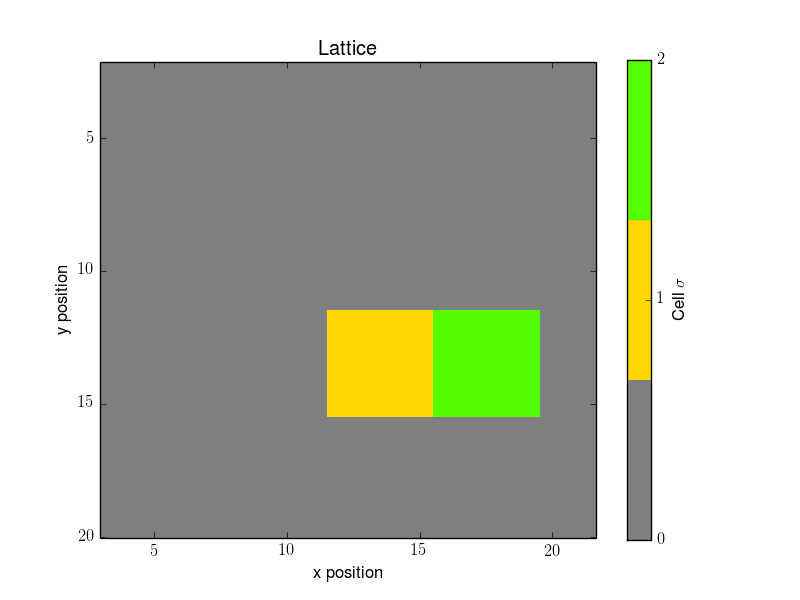
\includegraphics[scale=0.5]{img/basic}
	\caption{An example of two cells in a lattice, each color represents a different cell $\sigma$. The grey area is the Extra Cellular Matrix}
	\label{basic}
\end{figure}

\begin{figure}[H]
	\centering
	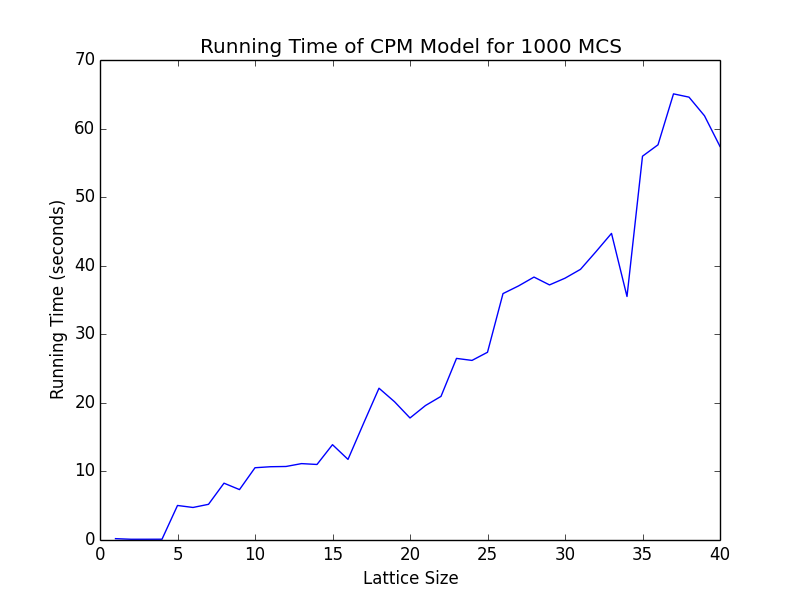
\includegraphics[scale=0.5]{img/runningtime}
	\caption{Running time for lattice size, $M =\{1,\ldots, 40\}$ and number of cells, $N=\frac{M^2}{25}$ for each simulation (average of three runs).}
	\label{runningtime}
\end{figure}

\pagebreak

\begin{figure}[H]
	\centering
	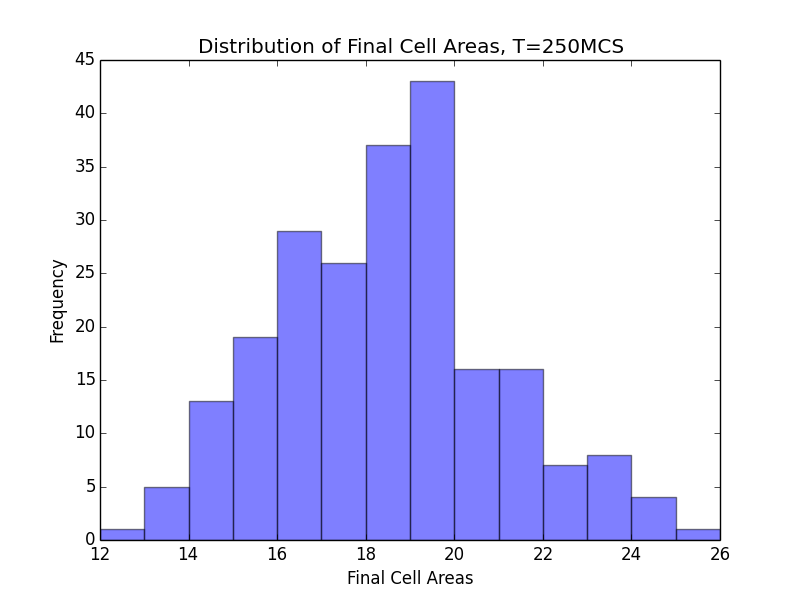
\includegraphics[scale=0.5]{img/cellareas}
	\caption{The distribution of final cell areas for $N=250$ simulations of a single-spin cell after $250$MCS. ($\mu = 17.99, \sigma^2=6.39$) }
	\label{cellareas}
\end{figure}

\begin{figure}[H]
	\centering
	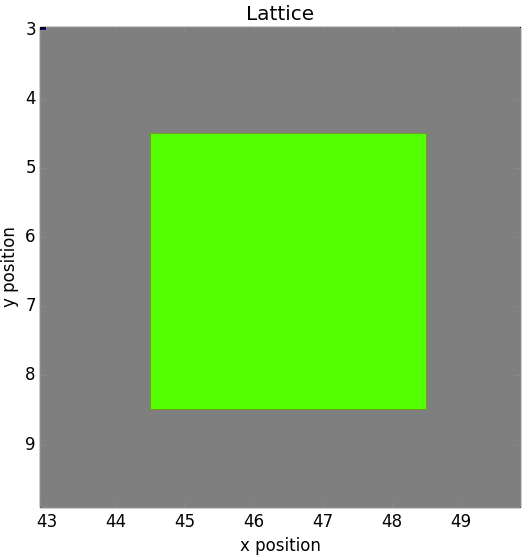
\includegraphics[scale=0.20]{img/1ctc_start}
	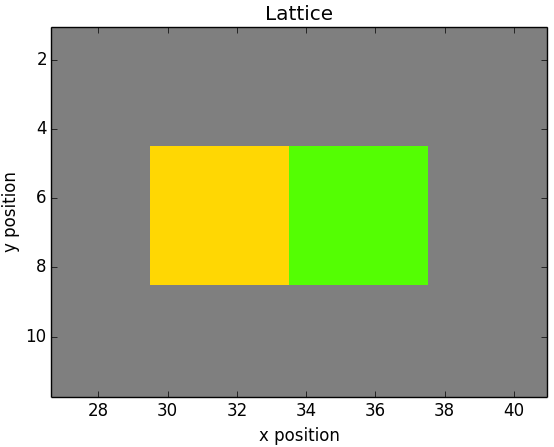
\includegraphics[scale=0.20]{img/2ctc_start}
	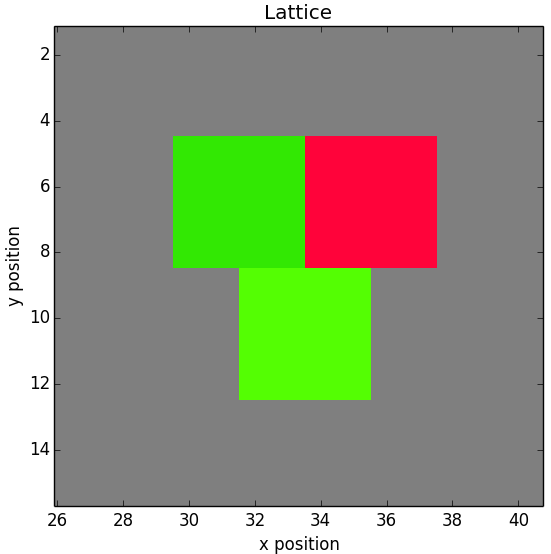
\includegraphics[scale=0.20]{img/3ctc_start}
	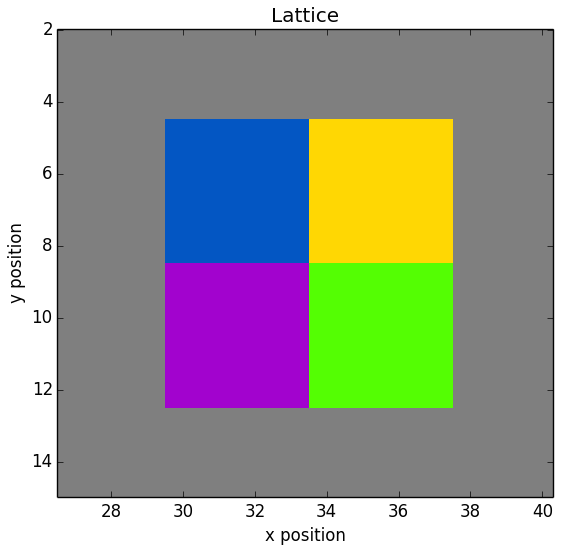
\includegraphics[scale=0.20]{img/4ctc_start}
	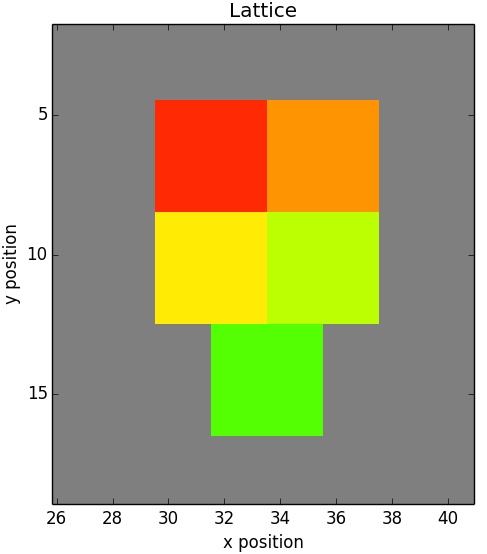
\includegraphics[scale=0.20]{img/5ctc_start}
	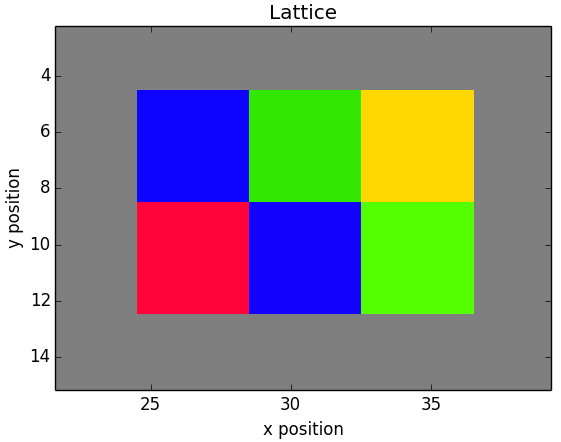
\includegraphics[scale=0.20]{img/6ctc_start}
	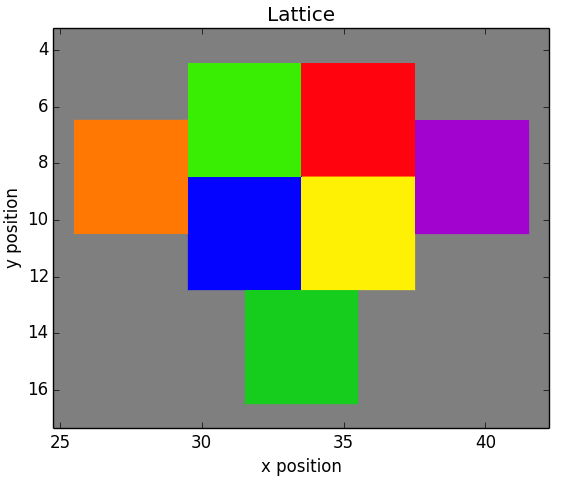
\includegraphics[scale=0.20]{img/7ctc_start}
	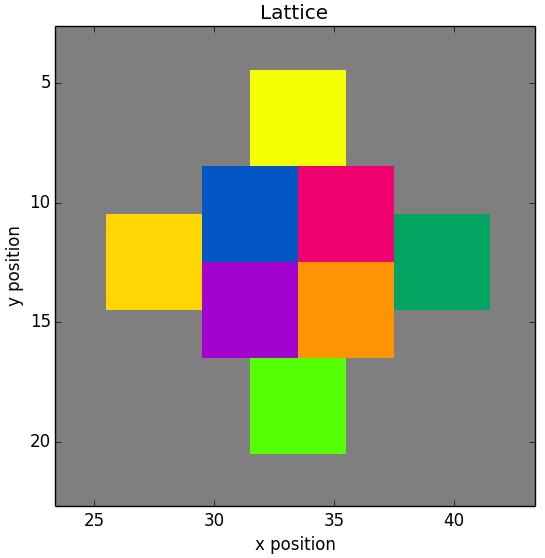
\includegraphics[scale=0.20]{img/8ctc_start}
	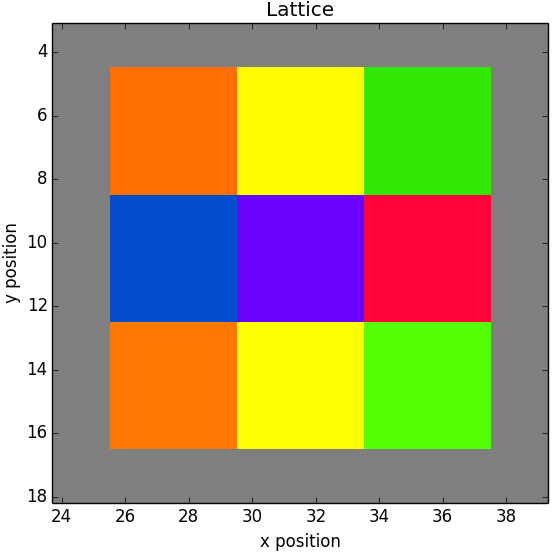
\includegraphics[scale=0.20]{img/9ctc_start}
	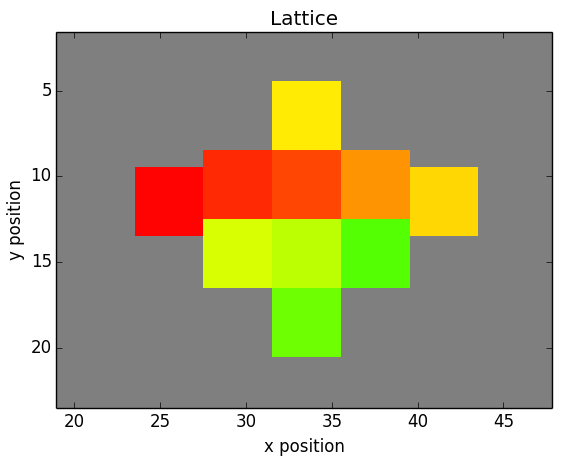
\includegraphics[scale=0.20]{img/10ctc_start}
	\caption{Starting positions of $k$-CTC for $10 \geq k \geq 1$.}
	\label{racestart}
\end{figure}

\begin{table}[H]
	\begin{tabular}{|l|l|l|l|l|l|l|l|l|l|l|}
	\hline
	k                                         & 1     & 2     & 3     & 4     & 5     & 6     & 7     & 8     & 9     & 10    \\ \hline
	Mean Velocity $(\frac{10^-3}{MCS})$ & 21.49 & 23.88 & 25.80 & 25.50 & 24.70 & 25.38 & 25.22 & 24.08 & 25.06 & 25.01 \\ \hline
	Variance in velocity 							& 22.89		&	7.44	&	7.24	&	0.91	&	1.47	&	0.47	&	0.72	&	1.07	&	1.07	&	1.70 \\ \hline
	Splitting Frequency              & N/A   & 0.2   & 0.06  & 0.02  & 0.03  & 0.00  & 0.01  & 0.01  & 0.02  & 0.01  \\ \hline
	Survival             & 1.00  & 1.00  & 1.00  & 1.00  & 1.00  & 1.00  & 1.00  & 1.00  & 1.00  & 1.00 \\ \hline
	\end{tabular}
	\caption{Results from running $k$-CTCs experiencing a constant force for successive $k$.}
	\label{racestats}
\end{table}
\pagebreak
\begin{figure}[H]
	\centering
	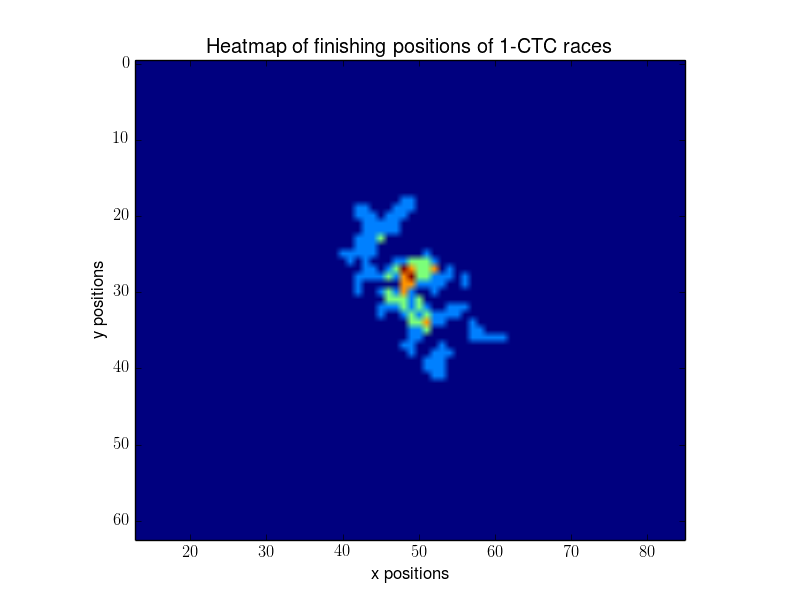
\includegraphics[scale=0.40]{img/1ctc_heat}
	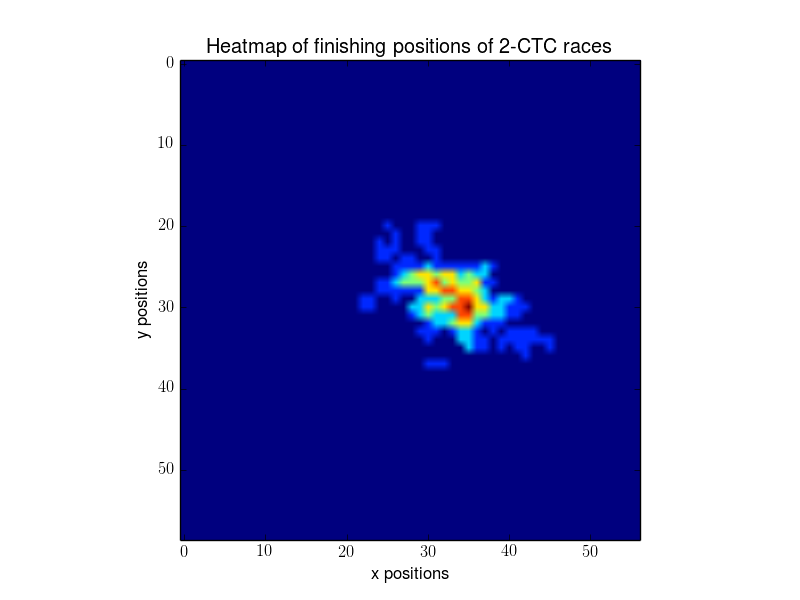
\includegraphics[scale=0.40]{img/2ctc_heat}
	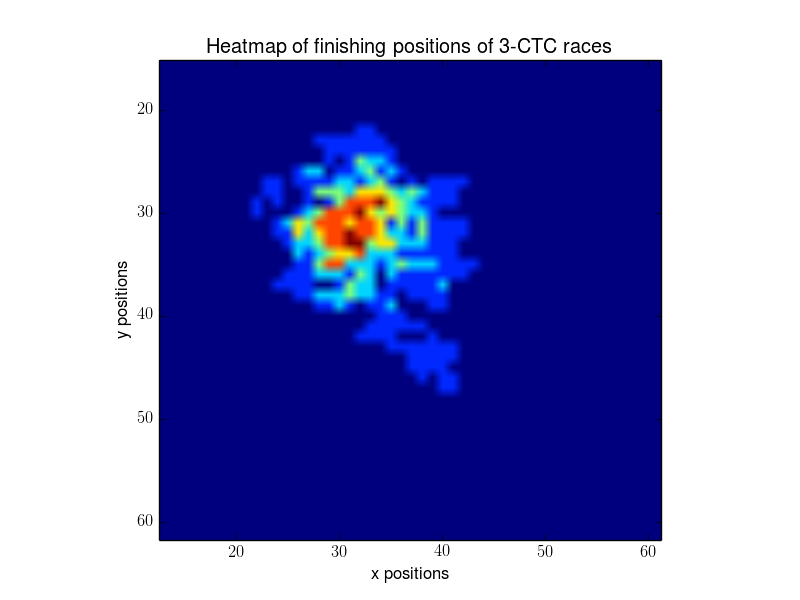
\includegraphics[scale=0.40]{img/3ctc_heat}
	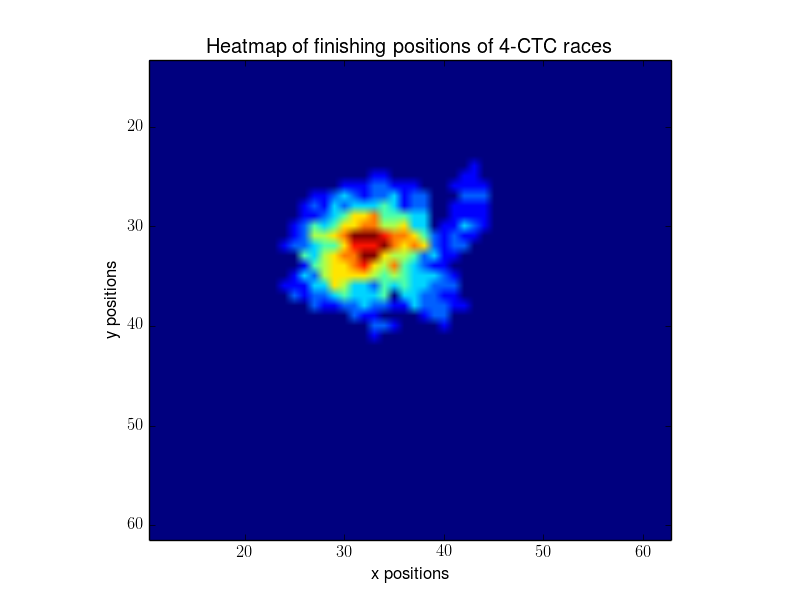
\includegraphics[scale=0.40]{img/4ctc_heat}
	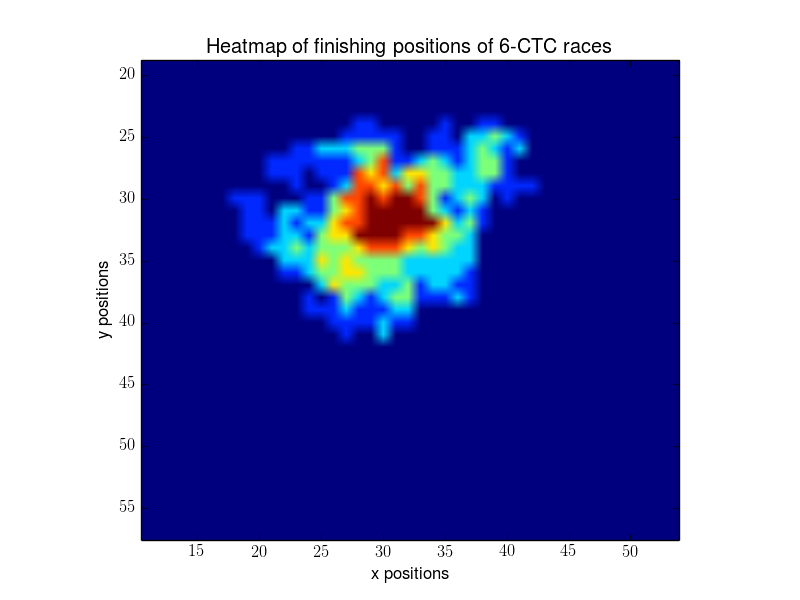
\includegraphics[scale=0.40]{img/6ctc_heat}
	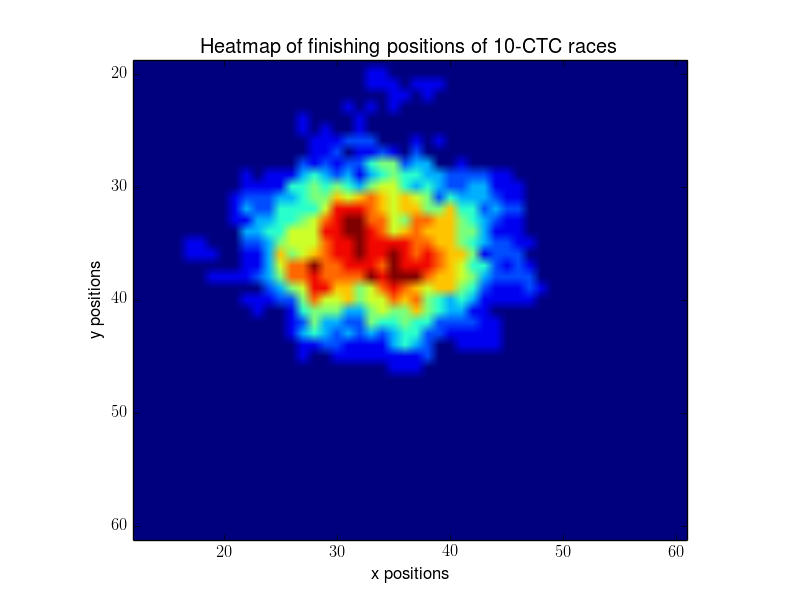
\includegraphics[scale=0.40]{img/10ctc_heat}
	\caption{Heatmaps for ending configurations of $k$-CTCs, $k\in\{1,2,3,4,6,10\}$. We can observe that $1$-CTCs and $2$-CTCs have a wider range of ending configurations while, $k=3,4,6,10$ move in more unison and have simillar ending configurations.}
	\label{heatmap}
\end{figure}

\begin{figure}[H]
	\centering
	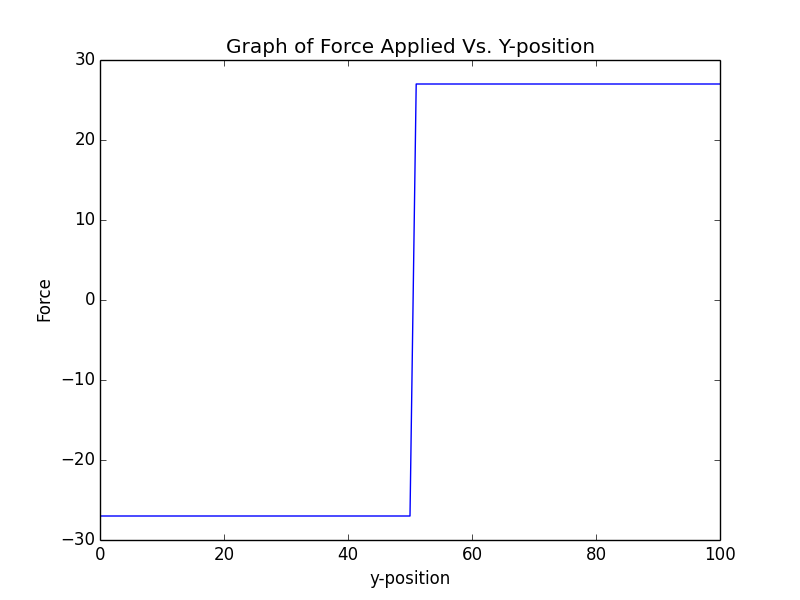
\includegraphics[scale=0.5]{img/forceapplied}
	\caption{Representation of the force applied at each y-position of the lattice. A positive force represents and acceleration in the positive $y$ direction.}
	\label{forceapplied}
\end{figure}

\begin{figure}[H]
	\centering
	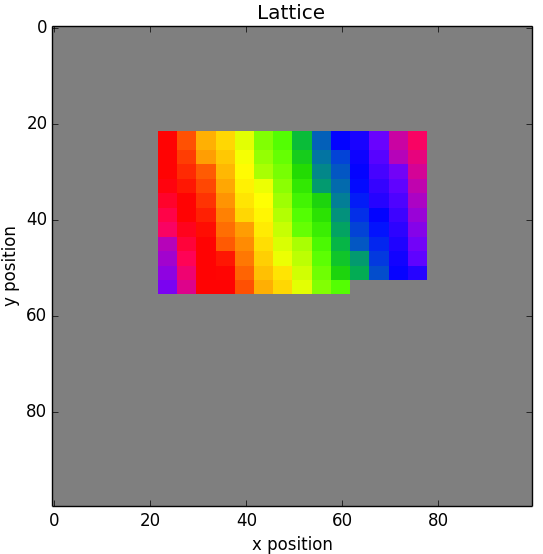
\includegraphics[scale=0.52]{img/nebula_0}
	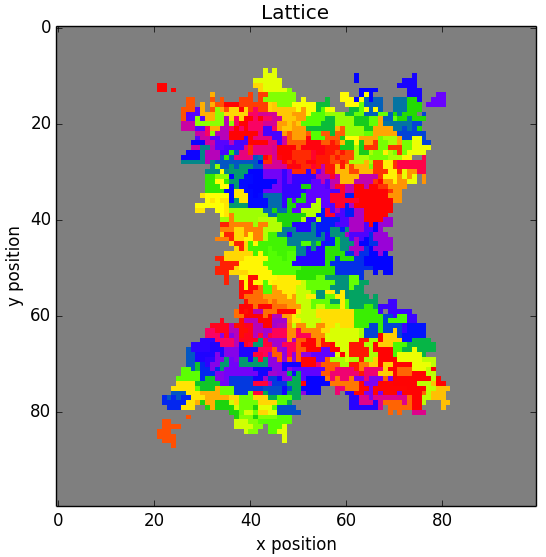
\includegraphics[scale=0.52]{img/nebula_5000}
	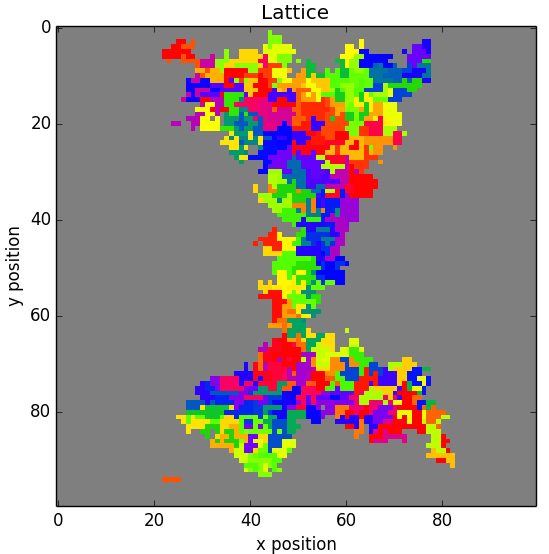
\includegraphics[scale=0.52]{img/nebula_9000}
	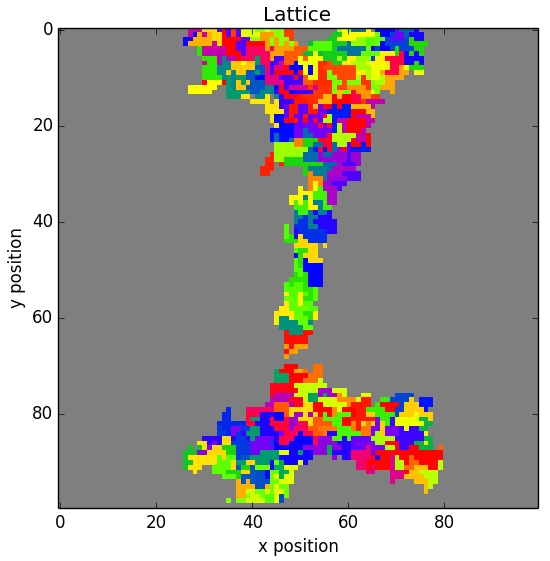
\includegraphics[scale=0.52]{img/nebula_13000}
	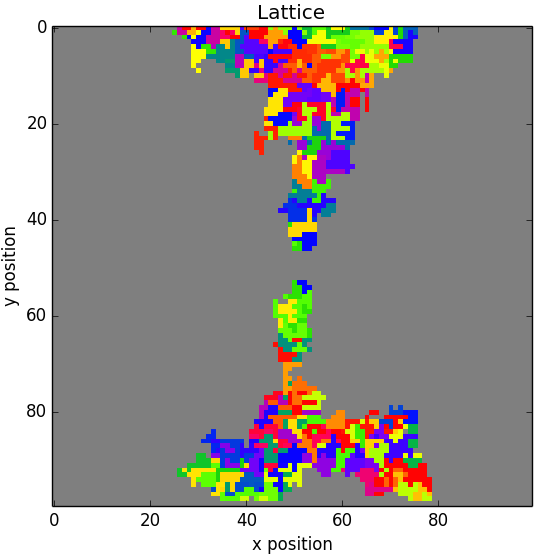
\includegraphics[scale=0.52]{img/nebula_15000}
	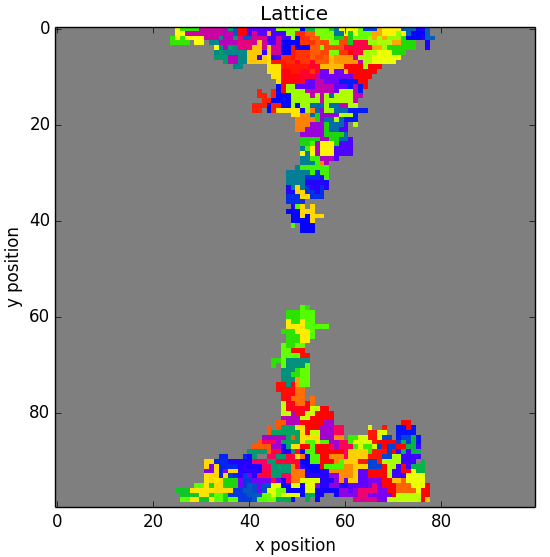
\includegraphics[scale=0.52]{img/nebula_17000}
	\caption{Time series representing the splitting of a Tissue into two by using a discontinous force. (From left to right, top to bottom: $t=0,5000,9000, 13000, 15000,17000)$}
	\label{nebula}
\end{figure}

\newpage
\bibliographystyle{abbrv}
\bibliography{396}


\end{document}